\documentclass[]{beamer}
\usepackage{lmodern}
\usepackage[ngerman]{babel}
\usepackage[utf8]{inputenc}
\usepackage[T1]{fontenc}
\usepackage{verbatim}
\usepackage{graphicx}
\usepackage[noend]{algpseudocode}

\usetheme{Frankfurt}



\title{Mehrgitter und konjugierte Gradienten Verfahren}
\author{Juri Schröder, Alexander Schmidt}
\date{\today}

\begin{document}


\begin{frame}
\titlepage
\end{frame}

\begin{frame}
\frametitle{Inhaltsverzeichnis}
\tableofcontents
\end{frame}


\section{Mehrgitter Verfahren}
\begin{frame}
  \frametitle{Mehrgitter}
  \begin{algorithmic}
    \Function{MG\_Iteration}{$N$, p, rhs}
    \State \Call{smooth}{$N$, p, rhs}
    \State res $\gets$ \Call{compute\_res}{$N$, p, rhs}
    \State res\_c $\gets$ \Call{restrict}{$N$, res}
    \If{$N \leq 8$}
    \State \Call{solve}{p, rhs}
    \Else
    \State e\_c $\gets$ \Call{MG\_Iteration}{$N/2$, e\_c, res\_c}
    \State e $\gets$ \Call{interpolate}{$N$, e\_c}
    \State p $\gets$ \Call{add}{p, e}
    \State \Call{smooth}{$N$, p, rhs}
    \EndIf
    \EndFunction
  \end{algorithmic}
\end{frame}

\begin{frame}
  \frametitle{Mehrgitter Konvergenz}
  \begin{center}
    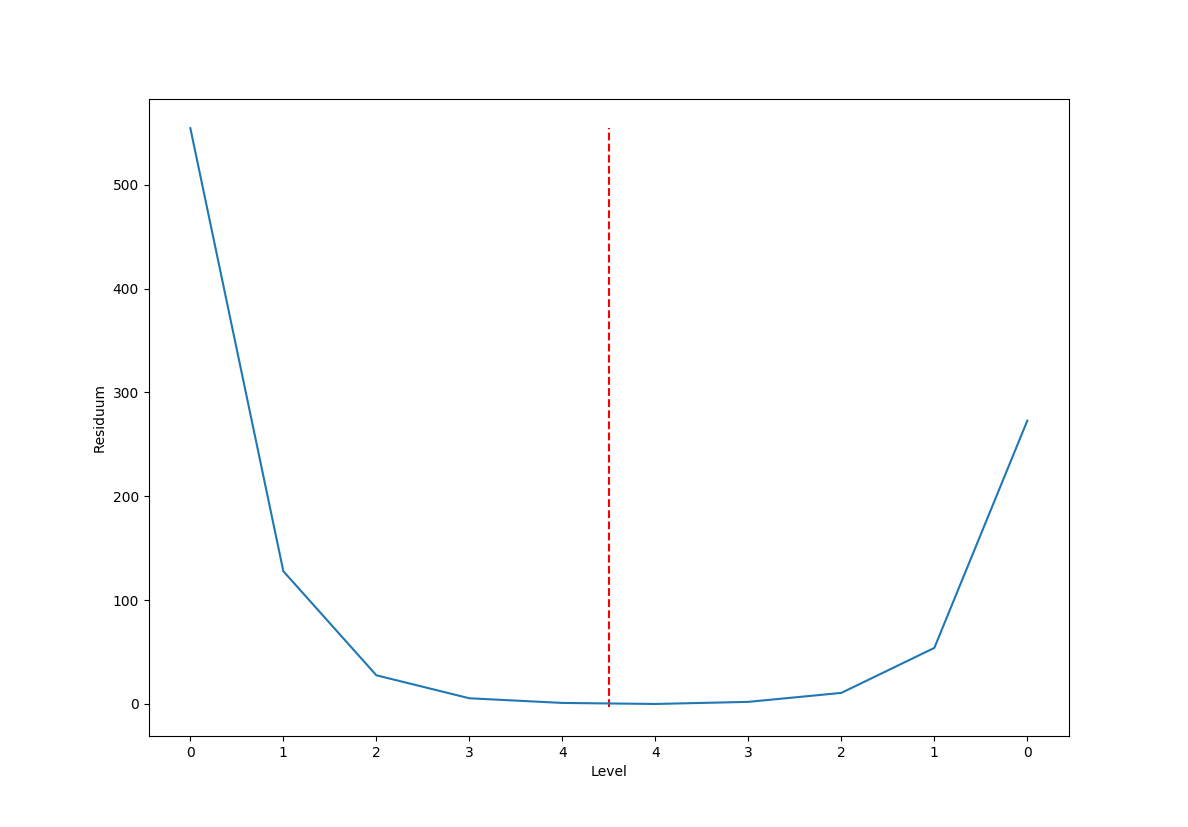
\includegraphics[width=0.9\linewidth, height=7cm]{MG_res_by_level.png}
  \end{center}
\end{frame}

\begin{frame}
  \frametitle{Mehrgitter Konvergenzanalyse}
  \begin{center}
    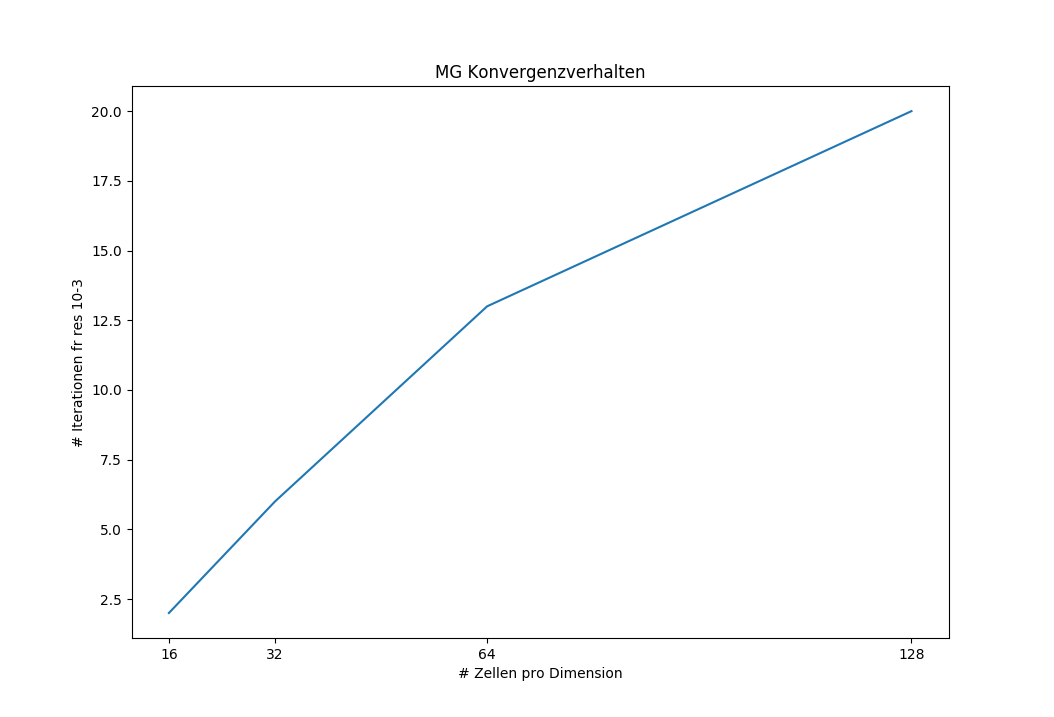
\includegraphics[width=0.9\linewidth, height=7cm]{mg_konvergenzverhalten.png}
  \end{center}
\end{frame}

\begin{frame}
  \frametitle{Vergleich mit SOR}
  \begin{center}
    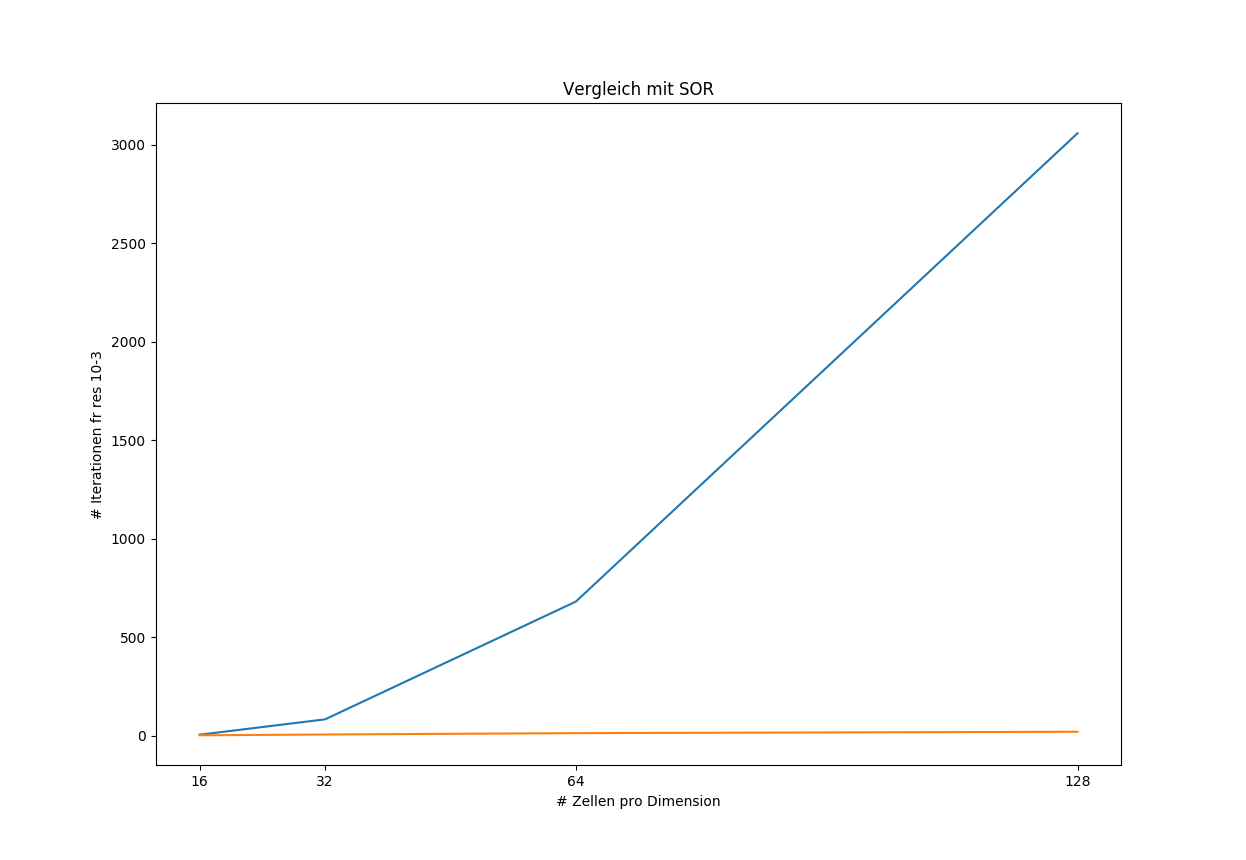
\includegraphics[width=0.9\linewidth, height=7cm]{mg_vs_sor.png}
  \end{center}
\end{frame}


\section{konjugierte Gradienten Verfahren}
\begin{frame}
\frametitle{Theorie}
$Ax = b,  $\, mit\, $ A \in \mathbb{R}^{n \times n}$ positive-definit und symmetrisch, $ b \in \mathbb{R}^n$
\\
Wähle $x_0 \in \mathbb{R}^n$
\\
$r = b - A x$
\\
$ d = r$
\\
while( $\| r \| < tol $ )
\\
\hspace*{1cm} $ z = Ad$
\\
\hspace*{1cm} $\alpha = \frac{ r^T r}{d^T z}$
\\
\hspace*{1cm} $x = x + \alpha d$
\\
\hspace*{1cm} $ c = r^T r$
\\
\hspace*{1cm} $r = r - \alpha z$
\\
\hspace*{1cm} $\beta = \frac{ r^T r}{ c }$
\\
\hspace*{1cm} $d = r + \beta d$
\\
end while
\end{frame}

\begin{verbatim}
  for( it.First(); it.Valid(); it.Next() ){
     Ad->Cell( it ) = _direction->dxx( it ) + _direction->dyy( it ); }
\end{verbatim}

\begin{frame}
\frametitle{Konvergenzverhalten}
\begin{center}
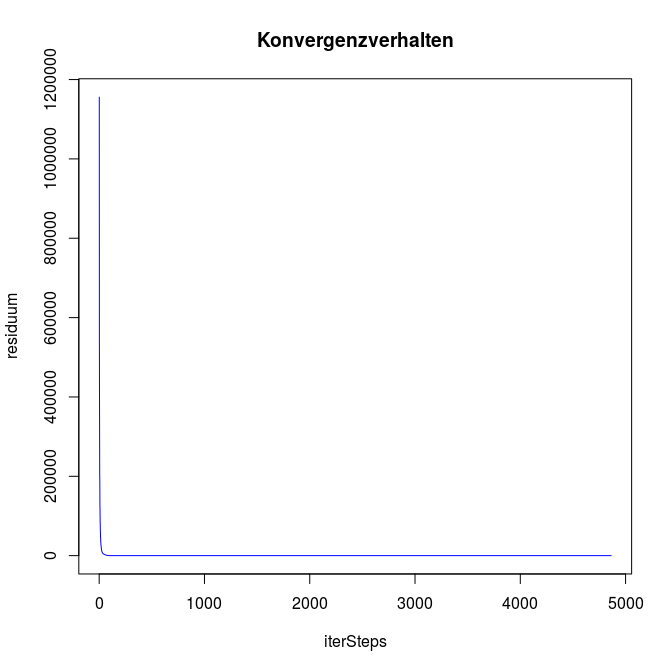
\includegraphics[scale=0.3]{Konvergenzverhalten_ganz.png}
\end{center}
\end{frame}

\begin{frame}
\frametitle{Konvergenzverhalten}
\begin{center}
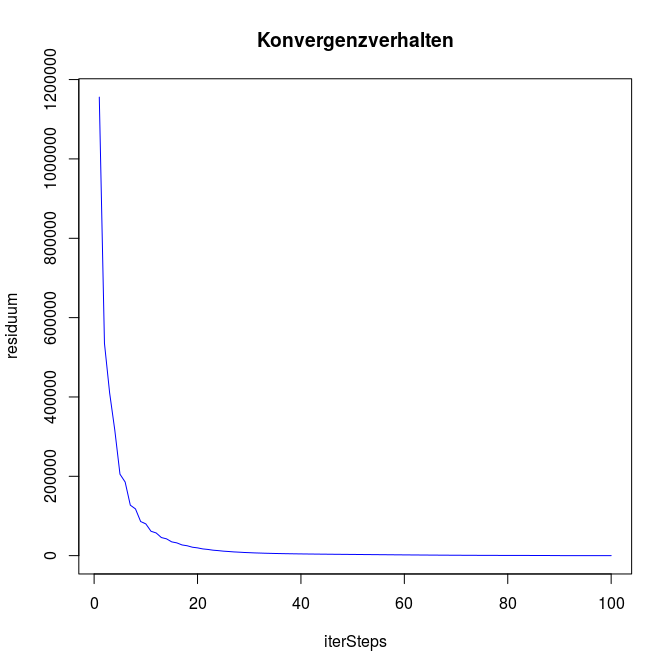
\includegraphics[scale=0.33]{Konvergenzverhalten_1_100.png}
\end{center}
\end{frame}

\begin{frame}
\frametitle{Konvergenzverhalten}
\begin{center}
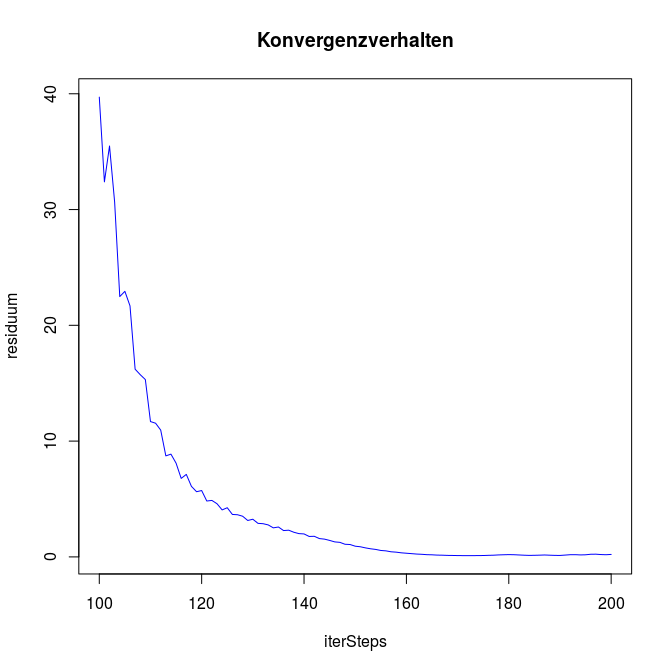
\includegraphics[scale=0.33]{Konvergenzverhalten_100_200.png}
\end{center}
\end{frame}

\begin{frame}
\frametitle{Konvergenzverhalten}
\begin{center}
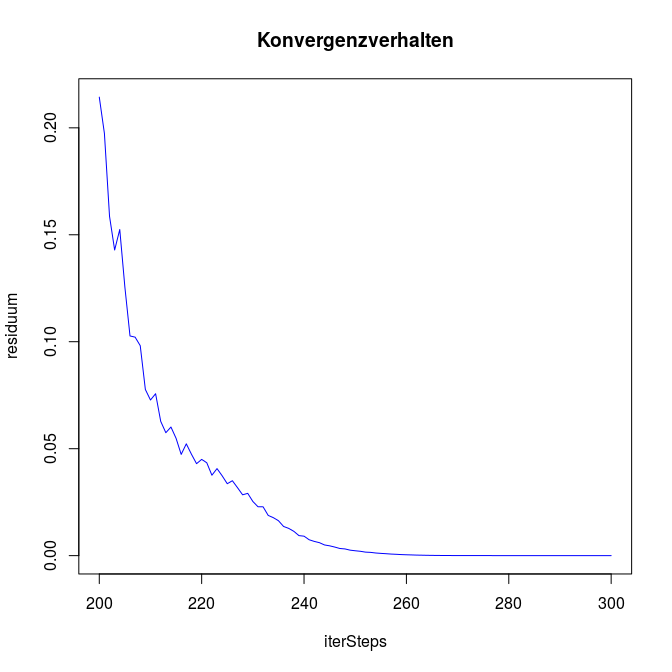
\includegraphics[scale=0.33]{Konvergenzverhalten_200_300.png}
\end{center}
\end{frame}

\begin{frame}
\frametitle{Konvergenzverhalten}
\begin{center}
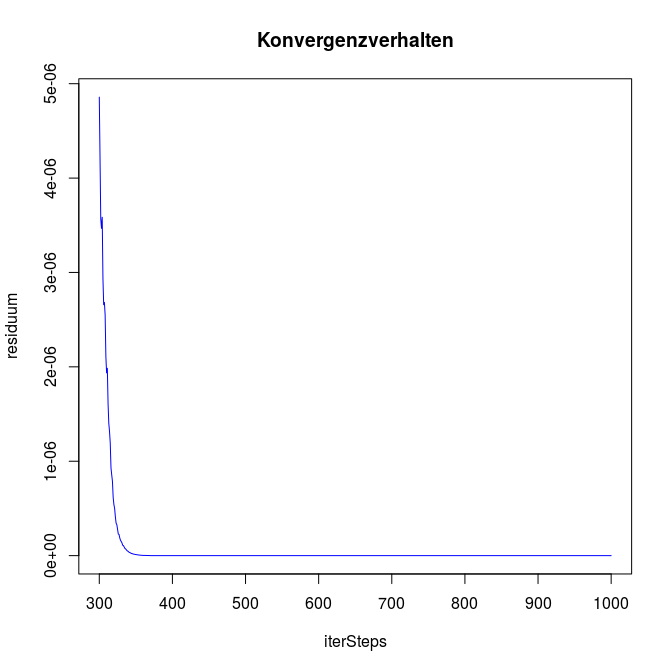
\includegraphics[scale=0.33]{Konvergenzverhalten_300_1000.png}
\end{center}
\end{frame}

\end{document}
